
%6%%6%%6%%6%%6%%6%%6%%6%%6%%6%%6%%6%%6%%6%%6%%6%%6%%6%%6
%                     Validação                        %
%6%%6%%6%%6%%6%%6%%6%%6%%6%%6%%6%%6%%6%%6%%6%%6%%6%%6%%6

\chapter{Estudo de validação}

\label{chap:evaluation}

Para avaliar a estratégia que apresentamos no Capítulo \ref{chap:metrics}, conduzimos um estudo empírico a fim de analisar se as métricas que propomos são capazes de identificar as soft skills dos indíviduos que utilizam o juiz online Huxley.

Neste estudo, estamos levando em consideração a relação que existe entre as soft skills e os fatores de personalidade que discutimos na Capítulo \ref{chap:concepts}. Propomos comparar se o resultado obtido através da aplicação das métricas identificam as soft skills associadas aos fatores de personalidade de um indivíduo. Para isso, coletamos as métricas que detalhamos na Seção \ref{sec:metrics} para um grupo de usuários do Huxley. Em seguida, os convidamos para responder um breve questionário a respeito de personalidade, com o objetivo de comparar os resultados. 

Para explicar o estudo de validação, apresentamos os participantes e o material na Seção \ref{sec:participantes} e Seção \ref{sec:material}, respectivamente. Então, na Seção \ref{sec:procedimento} detalhamos o procedimento que seguimos durante a avaliação das métricas para identificação de soft skills.

\section{Participantes}
\label{sec:participantes}

Os participantes do estudo de validação são usuários do Huxley e estudantes matriculados nas disciplinas de Programação dos cursos de Ciência da Computação e Engenharia da Computação, na Universidade Federal de Alagoas. A Tabela \ref{tab:participantes} distribui o número de participantes por semestre e curso:

\begin{table*}[h]
\footnotesize
\caption{\small Participantes}
\addtolength{\tabcolsep}{-3.5pt}
\renewcommand{\arraystretch}{1.7} 
\centering

\begin{tabular}{|c|c|c|}
\hline
\textbf{Semestre} & \textbf{Curso} 		& 	\textbf{Número de estudantes matriculados} \\ \hline
2014.01 & Ciência da computação 	 		& 	33 		\\ \hline
2014.01 & Engenharia da computação 		& 	23 		\\ \hline
\multicolumn{2}{|c|}{\textbf{Total}} 	&		56 		\\ \hline
\end{tabular}

\label{tab:participantes}
\end{table*}

Durante as aulas de Programação, os professores repassavam problemas do Huxley para serem resolvidos como execício. Os estudantes também foram fortemente incentivados a submeter soluções para o sistema como atividade extra-classe, para praticar e aprender programação. O uso do Huxley foi obrigatório para atividades avaliativas, compondo parcialmente a nota de desempenho na disciplina.

\section{Material}
\label{sec:material}

O material utilizado nesse estudo consiste de mais de 450 problemas de programação contidos na base de dados do Huxley. Esses problemas estão disponíveis para qualquer usuário do sistema, e portanto, para todos os participantes.

Utilizamos ainda a base de dados do Huxley para coletar as métricas, com base no histórico de participação dos usuários participantes, considerando o período dos seis primeiros meses de uso do sistema. De forma geral, juntos os participantes enviaram 18.234 submissões para 326 problemas de programação do Huxley. Dessas submissões, 5.796 foram avaliadas como soluções corretas.

Convidamos os participantes para responder um questionário a respeito de personalidade, chamado TIPI – Ten Item Personality Inventory \cite{gosling:03}. Esse questionário foi proposto contendo apenas 10 itens como uma medida breve dos Cinco Fatores de personalidade, tratamos desse modelo (FFM) na Seção \ref{sec:ffm}. De acordo com os autores, o TIPI pode ser utilizado como alternativa a instrumentos longos, como o NEO PI-R, que contém 240 itens. Isso nos oferece mais espaço e tempo para focar no que está mais diretamente relacionado a nossa pesquisa, ou seja, as soft skills. Na Figura \ref{fig:tipi}, observe o questionário TIPI em sua versão original.

\begin{figure}[h*]
\centering
\caption{\small Ten-Item Personality Inventory (TIPI)}
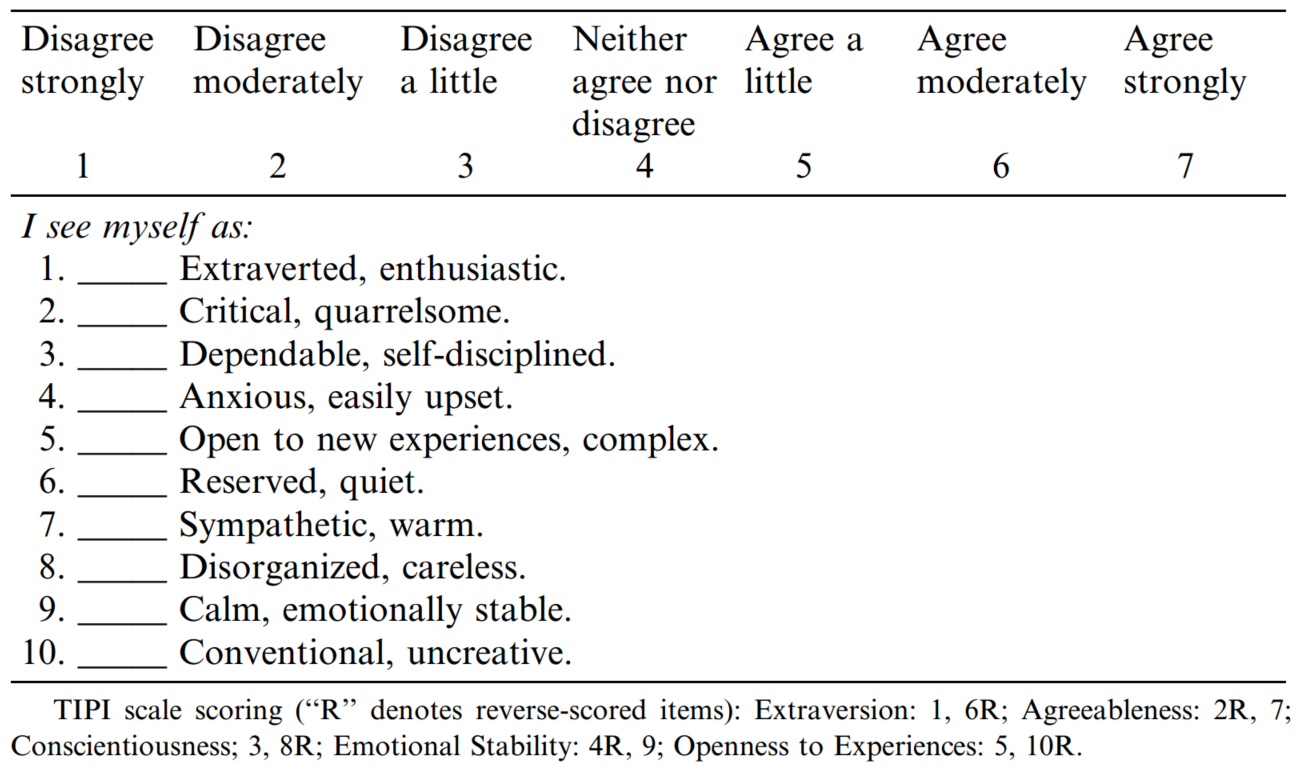
\includegraphics[width=.9\textwidth]{tipi.png}
\label{fig:tipi}
\fonte{\cite{gosling:03}}
\end{figure}

\section{Procedimento}
\label{sec:procedimento}

No primeiro passo do estudo de validação, coletamos as métricas que detalhamos na Seção \ref{sec:metrics} para cada participante utilizando a base de dados do Huxley. O período que consideramos para a coleta das dados inicia-se na data de cadastro do usuário. A partir dessa data, analisamos a participação do usuário, segundo a Tabela \ref{tab:dadosmetricas}, durante seis meses de uso do sistema. Esse período foi definido de acordo com o tempo do curso de programação, período no qual os usuários mais utilizam o Huxley.%, que é de um semestre.

Em seguida, preparamos o questionário TIPI para aplicá-lo ao grupo de participantes. O TIPI foi traduzido para português buscando-se manter o significado de cada item. A fim de esclarecer o objetivo do questionário, também foram adicionadas informações contextuais junto aos itens. Essas informações adicionais tratam-se de frases curtas que permitem ao participante entender que suas respostas devem ser dadas de acordo com seu comportamento enquanto pratica atividades de programação. Como recomendado por \cite{john:99}, adicionar esclarecimentos ou informações contextuais em instrumentos curtos é importante para evitar problemas de mal-entendimento, como ambiguidade ou significados múltiplos.
O Apêndice \ref{ap:tipi} apresenta o instrumento que aplicamos durante este estudo de validação, podemos ler os itens do TIPI e as informações contextuais que adicionamos.

O questionário TIPI foi aplicado presencialmente e individualmente para os participantes do estudo. O TIPI foi aplicado na última semana de aulas das disciplinas de Programação, ou seja, no mesmo período de tempo que as métricas das soft skills foram coletadas, no final do semestre. Nem todos os participantes estavam presentes, apenas 32 deles responderam o questionário. Em geral, nessa fase da disciplina, os estudantes estão em menor número, pois muitos deixam de ir para as aulas ou mesmo desistem. Apesar de termos coletado as métricas para todos os matriculados, apenas os dados dos que responderam o questionário TIPI participam da verificação dos resultados.
%Mesmo porque, não faz sentido considerar soft skills de programador daqueles que nem sequer finalizaram a disciplina.

Então, para atingir o objetivo deste estudo, verificamos se os resultados que encontramos aplicando as métricas correspondem aos resultados do questionário.
Para isso, estamos considerando o coeficiente de correlação de Pearson entre as pontuações das soft skills e pontuações do teste de personalidade.
Baseamos esse estudo, na relação que existe entre as soft skills e os fatores de personalidade que discutimos na Capítulo \ref{chap:concepts}.

Nossa hipótese é a seguinte: Uma métrica para identificação de soft skill pode ser validada se a mesma avalia sua respectiva soft skill em um nível que condiz com os traços de personalidade do indíviduo. Isso porque, se o indíviduo possui um determinado traço de personalidade, ele tende a possuir as soft skills relacionados a esse traço.
